\section{Theorie}
\label{sec:Theorie}
Genauer betrachtet wurde der Übergang von flüssig zu gasförmig. Dieser Teil der Kurve wird als
Dampfdruckkurve bezeichnet, er wird begrenzt durch den Tripelpunkt TP, bei dem alle drei Zustände
bei relativ niedriger Temperatur und niedrigem Druck parallel vorliegen, und dem kritischen
Punkt KP, bei dem (bei hoher Temperatur und hohem Druck) der Unterschied zwischen flüssiger und
gasförmiger Phase praktisch verschwindet.Gemessen wird dabei der Anstieg des sogenannten Sättigungsdampfdrucks,
der Druck, der vorliegt, wenn sich die Moleküle aus der flüssigen Phase und der Dampfphase in einem 
Gleichgewichtszustand befinden, bei dem sich die selbe Anzahl an Molekülen aus der Flüssigkeit löst wie 
Moleküle wieder eingefangen werden. Erhöht sich die Temperatur, so wird sich auch der Sättigungsdampfdruck 
erhöhen, da die Teilchengeschwindigkeiten größer werden und so mehr Moleküle aus der Flüssigkeit in die 
Dampfphase übergehen. \\
Die sogenannte molare Verdampfungswärme L ist eine Größe, die für jeden Stoff spezifisch und von der 
Temperatur abhängig ist; allerdings bestimmt die Verdampfungswärme auch den Verlauf der 
Dampfdruckkurve. Sie ist die Energie, die nötig ist, um einen Mol Flüssigkeit einer Substanz 
in Dampf mit derselben Temperatur umzuwandeln. Da sich bei einer Verdampfung Moleküle aus der Flüssigkeit
lösen und so intermolekulare Bindungskräfte überwinden müssen, ist diese Energie nötig. \\
Für einen bestimmten Temperaturbereich und mithilfe einiger Annahmen lässt sich
L als Konstante annähern um so die Dampfdruckkurve zu bestimmen. \\

\subsection{Herleitung der Differentialgleichung für die Dampfdruckkurve}
Es soll ein Kreisprozess betrachtet werden, in dem ein Mol eines Stoffes isotherm und isobar verdampft, 
woraufhin er isotherm und isobar kondensiert. Dabei ändert sich das Volumen des Stoffes. Temperatur
und Druck ändern sich zwischen den jeweiligen Vorgängen wie in Abbildung \ref{fig:kreis} dargestellt.
\begin{figure}
    \centering
    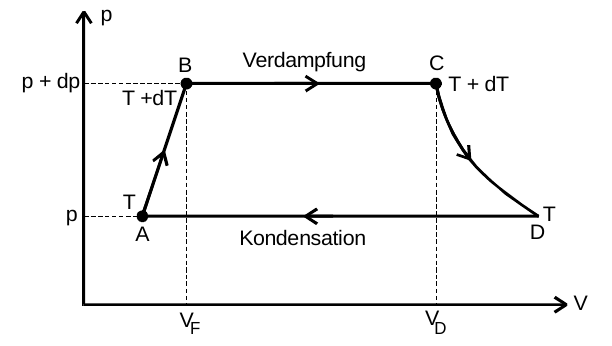
\includegraphics[width=\textwidth]{kreisprozess.png}
    \caption{Theoretischer reversibler Kreisprozess zur Herleitung der DGL.(Quelle [1])}
    \label{fig:kreis}
\end{figure}
Der Ausgangszustand, in der Abbildung als Punkt A dargestellt, ist die Flüssigkeit vorhanden mit 
Temperatur T und Druck p; um Zustand B zu erreichen, muss eine Wärmemenge $\symup{dQ_\text{AB}}$
zugeführt werden. In B hat die Flüssigkeit den Druck $\symup{p + dp}$ und die Temperatur $\symup{T + dT}$.
Wenn $\symup{c_F}$ die Molwärme der Flüssigkeit bezeichnet, gilt für die Wärmemenge:
\begin{equation*}
\symup{Q_\text{AB}}  = \symup{c_F dT}
\end{equation*}
Die Verdampfung wird durch Zufuhr der Verdampfungswärme eingeleitet, für die gilt:
\begin{equation*}
\symup{L \left( T + dT \right)} = \symup{L(T)} + \symup{dL}
\end{equation*}
Für diesen Vorgang muss von der Substanz eine Arbeit verrichtet werden, für die bei einer Vergrößerung
des Volumens von $\symup{V_F}$ für die Flüssigkeit und $\symup{V_D}$ für den Dampf gilt
\begin{equation*}
\symup{A_\text{BC}} = \left( \symup{p} + \symup{dp} \right) \left( \symup{V_D} - \symup{V_F} \right)
\end{equation*}
Um den Druck wieder auf die Temperatur T abzukühlen, wird dem Dampf die Wärmemenge
\begin{equation*}
\symup{dQ_\text{CD}} = \symup{C_D dT}
\end{equation*}
entzogen, wobei $\symup{C_D}$ die Molwärme des Dampfes bezeichnet. Das System kehrt zum Anfangszustand
zurück, indem der Dampf mithilfe mechanischer Energie komprimiert und so kondensiert wird. Dazu ist 
eine Arbeit nötig mit
\begin{equation*}
- \symup{A_{\text{DA}}} = \symup{p} \left( \symup{V_D} - \symup{V_F} \right)
\end{equation*}
Um die gesamte Wärme zu erhalten, die dem System zugeführt wurde, werden die beidem Wärmemengen und
die molare Verdampfungswärme summiert, es ergibt sich:
\begin{equation*}
\symup{dQ_\text{ges}} = \symup{c_F dT} - \symup{c_D dT} + \symup{L}(\symup{T}) + \symup{dL} - \symup{L(T)}
\end{equation*}
Nun ist nach dem Ersten Hauptsatz der Thermodynamik bekannt, dass in einem abgeschlossenen System die Wärmemenge gleich der verrichteten Arbeit 
sein muss.\\
Für die gesamte Arbeit, die verrichtet wurde, ergibt sich durch Summation:
\begin{equation*}
\symup{A_\text{ges}} = \symup{dp} \left( \symup{V_D} - \symup{V_F} \right)
\end{equation*}
Durch Gleichsetzen folgt:
\begin{equation}
\symup{c_F dT} - \symup{c_D dT} + \symup{L}(\symup{T}) + \symup{dL} - \symup{L(T)} = \symup{dp} \left( \symup{V_D} - \symup{V_F} \right)
\label{eqn:ersterHS}
\end{equation}
Nun ist aufgrund der Reversierbarkeit des Prozesses auch der zweite Hauptsatz der
Thermodynamik von Nutzen; demnach verschwindet auch die Summe der reduzierten
Wärmemengen $\frac{\symup{Q_i}}{\symup{T_i}}$:
\begin{equation}
\symup{\frac{c_F dT}{T} + \frac{L + dL}{T + dT} - \frac{c_D dT}{T} + \frac{L}{T}} = 0
\label{eqn:zweiterHS}
\end{equation}
Unter der Ahnnahme, dass dL und dT klein sind, können deren höhere Potenzen 
vernachlässigt werden und es gilt
\begin{equation*}
\symup{\frac{L + dL}{T + dT}} = \symup{\frac{L}{T} + \frac{dL}{T} - \frac{L dT}{T^2}}
\end{equation*}
Also folgt für \eqref{eqn:zweiterHS} nach Multiplikation mit T:
\begin{equation*}
\left( \symup{c_F - c_D} \right) dT + \symup{dL} - \frac{L dT}{\symup{T}} = 0
\end{equation*}
Mit Gleichung \eqref{eqn:ersterHS} lässt sich dL eliminiern, sodass sich ergibt
\begin{equation}
    \left( \symup{ V_D - V_F} \right) dp = \frac{L}{T} dT
    \label{eqn:clausius}
\end{equation}
\eqref{eqn:clausius} ist die gesuchte Differentialgleichung, die Clausius-Clapeyronsche
Gleichung. Mithilfe einiger Näherungsannahmen lässt sich durch diese Gleichung
für bestimmte Temperaturbereiche die Dampfdruckkurve einer Substanz berechnen. Im 
allgemeinen Fall ist sie allerdings weniger hilfreich, da sich dann wegen teilweise
komplexen Ausdrücken für die Volumen und die molare Verdampfungswärme die Integration
als zu schwierig herausstellt.

\subsection{Integration der Gleichung}
Unter der Voraussetzung, dass die kritische Temperatur $\symup{T_\text{kr}}$ viel größer
ist im Vergleich zur tatsächlichen Temperatur, können die zuvor erwähnten komplexen
Ausdrücke für die Volumina und Verdampfungswärme vereinfacht und so die Intgration 
leicht ermöglicht werden. Dann gelten:
\begin{enumerate}
    \item $\symup{V_F} << \symup{V_D}$
    \item $\symup{V_D} = R \frac{T}{p}$
    \item L ist druck- und temperaturunabhängig
\end{enumerate}
Es ergibt sich für \eqref{eqn:clausius}
\begin{equation*}
\frac{R}{p} dp = \frac{L}{T^2} dT
\end{equation*}
Die Integration gelingt so ohne Probleme. Also ist
\begin{equation}
\symup{ln(p)} = - \frac{L}{R} \frac{1}{T} + \symup{const}\\
\iff \symup{p} = \symup{p_0 \cdot exp \left( - \frac{L}{R} \cdot \frac{1}{T} \right)}
\end{equation}
